%!TEX root=../oi-magistr-spolecne.tex
\section[KO - SPT, TSP, knapsack]{Nejkratší cesty. Úloha obchodního cestujícího. Heuristiky a aproximační algoritmy. Metoda dynamického programování. Problém batohu. Pseudo-polynomiální algoritmy.}

\subsection{Problém nejkratší cesty}

Nejkratší cesta je problém nalezení nejkratší cesty z $x$ do $y$. V obecném grafu se zápornými cykly je to NP-úplná úloha.

\paragraph{Bellmanova rovnice:} Polynomiální řešení problému nejkratších cest je založeno na Bellmanovu principu optimality, který říká, že \textbf{pokud} graf \textbf{neobsahuje cyklus záporné délky}, tak pro každé tři vrcholy $x, y, z$ platí:

$$u(x, y) = \min_{x \neq y} (u(x, z) + a(z, y))$$

Kde $u(x, y)$ značí délku cesty z vrcholu $x$ do vrcholu $y$ a $a(z, y)$ značí vzdálenost vrcholu $z$ od vrcholu $y$ (tj. délku nejkratší hrany, která tyto vrcholy spojuje).

Z Bellmanovy rovnice jednoduše řečeno vyplývá, že se každá \textbf{nejkratší cesta skládá z nejkratších cest} – tj. nejkratší cesta $[a, \cdots , x, \cdots , c]$ mezi uzly $a$ a $b$ obsahuje také nejkratší cestu mezi uzly $a$, $x$ a $x$, $c$.

Polynomiální algoritmy pro nejkratší cesty:

\paragraph{Dijkstra: $O(E\cdot \log V)$} Funguje \textbf{pokud nejsou záporné hrany}. Algoritmus má uzly v prioritní frontě podle vzdálenosti od zdroje. Na začátku zdroj 0, ostatní nekonečno. Vždy odebere uzel s nejmenší vzdáleností a provede tzv. relaxaci - podívá se na všechny sousedy ještě ve frontě a ověří, jestli se tam přes tento uzel nejde dostat rychleji. Pokud ano, sníží prioritu. Když odebereme cílový uzel, algoritmus končí. Je dobré si zaznamenávat předchůdce.

\paragraph{Bellman-Ford: $O(E\cdot V)$} Podobný Dijkstrovi, ale funguje pro hrany záporné délky. Může také \textbf{detekovat záporný cyklus}. 

Základem Bellman-Fordova algoritmu je operace relaxace. Do této operace vstupují dva uzly a hrana, která mezi nimi vede. Pokud je vzdálenost zdrojového uzlu sečtená s délkou hrany menší než aktuální vzdálenost cílového uzlu, tak se za předchůdce cílového uzlu na nejkratší cestě označí zdrojový uzel (a vzdálenost cílového uzlu se přepočítá). V případě nesplnění nerovnosti tato hrana cestu nezkracuje a neprovádí se proto žádné změny.

Délka cesty ze zdrojového do každého z cílových uzlů může být dlouhá maximálně |V|-1 hran (protože by jinak musela obsahovat cyklus). Proto pokud pustíme operaci relaxace na všechny hrany grafu |V|-1 krát, tak již musí být nalezeny všechny nejkratší cesty. Toto ověříme ještě jedním spuštěním relaxací všech hran. Pokud dojde k nějaké relaxaci, tak graf obsahuje cyklus záporné délky, pokud k relaxaci nedojde, algoritmus může vrátit výsledek.

\paragraph{Floyd-Warshall: $O(E^2 \cdot V)$} Najde nejkratší cesty od všech uzlů ke všem, detekuje záporné cykly. Nejdřív matice kdo s kým sousedí, iteruju $k=1..n$. Procházím všechny prvky a dívám se co protínám v k-tém řádku a sloupci. Sečtu ty prvky. Když je součet menší, nahradím. Při náhradách je dobré vést matici předchůdců. Když bude $<0$ na diagonále - záporný cyklus.

\paragraph{Existence hamiltonovské kružnice} Je neorientovaný graf a máme rozhodnout, zda existuje HC (kružnice která navštíví každý vrchol přesně jednou). Je to \textbf{NP-úplný problém}.

\subsection{Úloha obchodního cestujícího (TSP)}

Problém je NP-úplný a silně NP-obtížný, což znamená, že pokud platí $P \neq NP$, pak pro problém obchodního cestujícího \textbf{neexistuje} žádný polynomiální \textbf{k-aproximační} algoritmus - neexistuje polynomiální algoritmus, který by našel libovolné řešení, které je nejhůře k-násobkem optimálního řešení.

\paragraph{Důkaz NP-hard:} \hl{Redukcí z existence Hamiltonovské kružnice.}

Mějme neorientovaný graf $G$, kde rozhodujeme jestli tam je hamiltonovská kružnice. Vytvoříme instanci TSP tak, že vytvoříme uplný graf $K$. Každý vrchol z $G$ je přiřazen jednomu vrcholu v $K$. Cena hran $\{i,j\}$ v $K$ je rovna:

\begin{align*}
c(\{i,j\})=\begin{cases}
    1 & \text{pokud hrana $\{i,j\}$ je v $G$}\\
    2 & \text{pokud hrana $\{i,j\}$ není v $G$}
  \end{cases}
\end{align*}

$G$ má hamiltonovskou kružnici právě tehdy, když optimální řešení TSP se rovná $n$. $\Rightarrow$ TSP je silně NP-hard.

\subsubsection{Metrický obchodní cestující}
Variantou tohoto problému je problém metrického obchodního cestujícího, ve kterém vzdálenosti na grafu splňují trojúhelníkovou nerovnost. Toto zjednodušení odpovídá velkému množství reálných problémů (např. hledání na mapě), a zároveň umožňuje konstrukci aproximačních algoritmů.

\paragraph{2-aproximační algoritmus:} \hl{Nalezne se kostra Kruskalem a vypíše se první výskyt uzlů při procházení do hloubky.}

Algoritmus nejprve zkonstruuje minimální kostru grafu. Z definice kostry plyne, že  cena(kostra) $\leq$ cena(optimum) protože kostra obsahuje $\vert V \vert -1$ minimálních hran, zatímco kružnice jich obsahuje $\vert V \vert$.

V druhém kroku projde algoritmus kostru z libovolného uzlu do hloubky a poznamená si všechny průchody přes vrcholy - protože se jedná o průchod do hloubky, budou zde některé uzly zpracovány vícekrát.

V posledním kroku - zkrácení cest - algoritmus tento seznam projde a vynechá všechny duplicity (zanechá pouze první výskyty uzlů). Tímto dojde k vytvoření samotné kružnice.

\begin{figure}[h]
    \begin{center}
        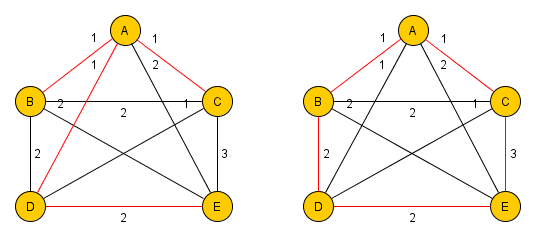
\includegraphics[width=100mm]{09/images/tsp-2aprox}
    \end{center}
    \caption{2-aproximační alg pro TSP: např. A,B,D,E,C}
\end{figure}

\paragraph{3/2-aproximační algoritmus (Christofidesův):}
Christofidesův algoritmus řeší problém metrického obchodního cestujícího tak, že je výsledná trasa v nejhorším případě dlouhá 3/2 délky trasy optimálního řešení. Toto zlepšení je ovšem vykoupeno výrazně obtížnější implementací, a zároveň se na reálných datech ukazuje, že výsledek není v průměrném případě o mnoho lepší než při použití 2-aproximačního algoritmu uvedeného výše.

Christofidesův algoritmus nejprve zkonstruuje \textbf{minimální kostru grafu}. Poté kostru \textbf{projde} z libovolného uzlu \textbf{do hloubky} a \textbf{vybere} ty \textbf{uzly}, jež mají \textbf{lichý stupeň} a zkonstruuje na nich \textbf{úplný graf} G. Na grafu G nalezne \textbf{nejlevnější perfektní párování} $P$. Hrany z $P$ přidá do minimální kostry. Graf $K \cup P$ je nyní \textbf{eulerovský} (tzn. existuje v něm tah, který obsahuje všechny hrany grafu). Algoritmus nyní nalezne eulerovský tah – výsledná trasa odpovídá pořadí prvních návštěv uzlů při konstrukci tohoto tahu.

\subsection{Batoh (Knapsack)}
Problém batohu (Knapsack) řeší problém, které předměty dát do batohu tak, aby nebyla překročena kapacita $W$ a celková cena $C$ byla maximální.

\paragraph{2-aproximační alg $O(n^2)$} Předpokladem je, že každý z předmětů má nižší váhu než je kapacita batohu $W$ (těžší můžeme vypustit). A součet těchto vah je naopak větší než kapacita batohu (kdyby měli menší nebo roven, tak již máme optimální řešení).

\begin{enumerate}
\item Seřadíme sestupně předměty podle jejich poměru cena/váha $\frac{c_i}{w_i}$
\item Z takto seřazených předmětů vezmeme nejmenší část předmětů $h$, která přeleze přes kapacitu $W$, tzn. $h = \min\{j \in \{1,\hdots n\} : \sum\limits^{j}_{i = 1} w_i > W\}$
\item Nakonec se vezme lepší ze dvou řešení $\{1,\hdots, h-1\}$ nebo $\{h\}$
\end{enumerate}

\subsection{Dynamické programování}
Algoritmus, kde jsou udržovány mezivýsledky (něco jako cache na výsledky), které jsou dále využívány.

\paragraph{Dynamické programování na problém batohu}
Dynamické programování může vyřešit pseudo-polynomiálně. Mám tabulku číslo rozhodnutí x váha. Vždy se větvím na dva - přidám nebo nepřidám. Posunu se dolů o 1 a vpravo kolik tím přibyde váhy. Když překročím kapacitu, ořez. Do políček zapisuju celkovou cenu. Když už na políčku něco je, nahrazuji jenom menší cenu. Nejvíc vpravo dole bude optimální řešení.

\begin{figure}[h]
    \begin{center}
        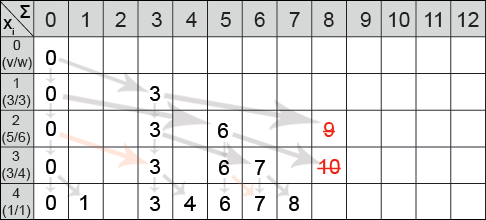
\includegraphics[width=100mm]{09/images/knapsack}
    \end{center}
    \caption{Batoh o kapacitě 8 a předměty s váhami: $[3,6,4,1]$, hodnotami $[3, 5, 3, 1]$}
\end{figure}

\subsection{Pseudo-polynomiální algoritmy}
Pseudo-polynomiální algoritmy mají složitost $O(c \cdot n)$, kde $c$ nezáleží na velikosti instance ($n$) a může být hodně velké, až exponenciální. Např. algoritmus dynamického programování pro Knapsack.
